68. \begin{figure}[ht!]
\center{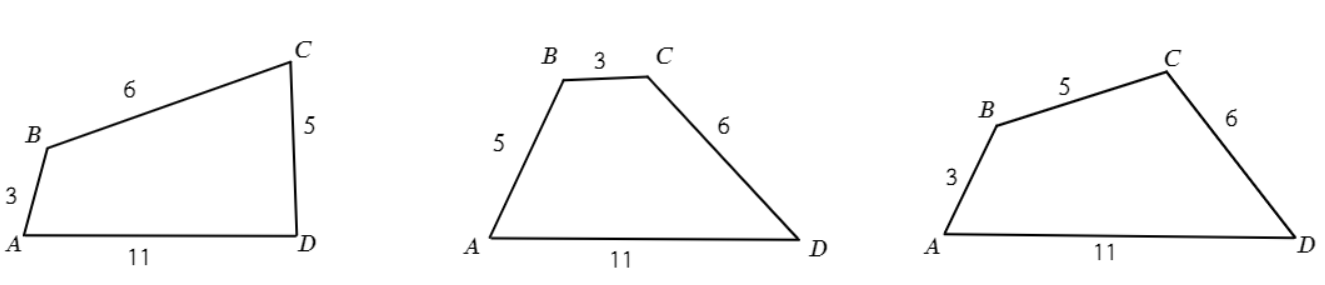
\includegraphics[scale=0.35]{g68.png}}
\end{figure}\\
Возможны три разных порядка расположения сторон этого четырёхугольника. Возможность существования четырёхугольника с заданными сторонами и целой диагональю определяется только выполнением неравенств треугольника для всех образовавшихся треугольников. Самое маленькое целое значение, которое может принимать диагональ --- это значение 6 для диагонали $AC$ во втором случае. Самое большое --- значение 10 для диагонали $BD$ в третьем случае. Значение 5 ни одна диагональ принимать не может, потому что она должна образовывать треугольник со стороной 11, а даже $5+6\leqslant11.$ Значение 11 ни одна диагональ принимать не может, потому что она должна образовывать треугольник без стороны 11, а даже $6+5\leqslant11.$ Таким образом, длина диагонали может принимать только значения $6,\ 7,\ 8,\ 9,\ 10.$\\
